\section{Calibration Methodology}
\label{sec:calibration_methodology}

The utility model in Eq.~\eqref{eq:utility} (directional alignment, speed alignment, proximity reward, collision penalty, and boundary adherence) contains ten free parameters
\[
\theta=\bigl(S_\theta,\,S_v,\,\xi_i,\,S_d,\,\gamma,\,w_x,\,w_y,\,w_c,\,w_\ell,\,\beta\bigr).
\]
These parameters are calibrated from the Lebanon naturalistic trajectory set so that the discrete utility prior reproduces observed short-horizon motion before any residual policy is trained.

\paragraph{Data and candidate actions.}
Valid passenger-vehicle transitions with time step $\Delta t\in[0.05,0.2]$\,s yield $190{,}767$ usable state records. From this pool we draw $N_{\mathrm{s}}=2000$ one-step choice samples. At each sample, the ego agent is reconstructed in the corridor frame with neighboring vehicles inside a $60$\,m radius (at most six neighbors). Candidate controls are generated on the same acceleration--steering grid used in simulation
(acceleration $\in\{-3,\ldots,3\}$\,m/s$^2$, steering $\in[-0.45,0.45]$\,rad), producing a discrete action set $\mathcal{A}$. The observed next state is matched to the nearest candidate (target index) for likelihood evaluation.

\paragraph{Closed-loop windows.}
Because one-step ranking alone under-constrains $\theta$, we additionally sample $N_{\mathrm{w}}=40$ short trajectory windows of horizon $H=8$ steps. From the observed initial state of each window, the utility model repeatedly selects $\arg\max_{a\in\mathcal{A}} U(a;\theta)$ and the simulated pose/speed/heading are compared with the recorded trajectory.

\paragraph{Objective.}
Calibration minimizes a weighted composite loss
\begin{equation}
\begin{aligned}
J(\theta)
&=
\lambda_{\mathrm{cl}}\,L_{\mathrm{cl}}(\theta)
+
\lambda_{\mathrm{trk}}\,\frac{\bar r(\theta)}{r_0}
+
\lambda_{\mathrm{nll}}\,L_{\mathrm{nll}}(\theta),
\end{aligned}
\label{eq:calibration_objective}
\end{equation}
where $L_{\mathrm{cl}}$ is the mean closed-loop tracking error (position, with speed and heading penalties), $\bar r$ is the mean rank of the observed-like candidate among $\mathcal{A}$, $r_0=63$ normalizes rank, and $L_{\mathrm{nll}}$ is the mean softmax negative log-likelihood of the target candidate at temperature $T=0.25$. We use $\lambda_{\mathrm{cl}}=1$, $\lambda_{\mathrm{trk}}=1$, and $\lambda_{\mathrm{nll}}=0.1$, so closed-loop fidelity is the primary target and the one-step likelihood acts as a light regularizer.

\paragraph{Search and robust aggregation.}
Because $J(\theta)$ is non-convex and partially flat, we do not trust a single optimizer trajectory. Parameters are drawn uniformly in the search box of Table~\ref{tab:utility_search_bounds}. For each of $R=3$ independent restarts (different random seeds), $N_{\mathrm{t}}=400$ vectors are screened by the cheap one-step terms; the best $80$ candidates per restart ($240$ scored trials in total) are then evaluated with the closed-loop windows. Let $\theta^\star$ be the minimizer of $J$ and define the near-optimal cloud as all scored trials with
\[
J(\theta)\le J(\theta^\star)+\max\bigl(0.05,\,0.05\,|J(\theta^\star)|\bigr).
\]
If fewer than three trials satisfy this cutoff, the top ten scored trials are used instead. The \emph{robust} working point $\theta_{\mathrm{rob}}$ is the coordinate-wise median of that cloud. This aggregation reduces sensitivity to isolated lucky minima while retaining the same predictive performance up to a small objective gap. Quantiles of the top/near-optimal clouds supply recommended ranges for subsequent global sensitivity analysis.

\begin{table}[t]
\centering
\caption{Search bounds used in utility calibration.}
\label{tab:utility_search_bounds}
\begin{tabular}{lcc}
\toprule
Parameter & Low & High \\
\midrule
$S_\theta$, $S_v$, $S_d$ & $0.05$ & $10$ \\
$\xi_i$ & $1.1$ & $10$ \\
$\gamma$, $\beta$ & $0.1$ / $0.01$ & $10$ \\
$w_x$, $w_y$ & $0.1$ & $10$ \\
$w_c$, $w_\ell$ & $0.01$ / $0.1$ & $1000$ \\
\bottomrule
\end{tabular}
\end{table}


\section{Calibration Results}
\label{sec:calibration_results}

\paragraph{Fit quality.}
Across the $2000$ choice samples, the selected utility prior places the observed-like candidate at median rank $8$ (mean $11.1$--$11.4$), with top-$5$ and top-$10$ hit rates of $35.7\%$ and $62.9\%$, respectively. The best scored trial attains $J(\theta^\star)=1.132$ (closed-loop loss $0.549$), while the robust median $\theta_{\mathrm{rob}}$ yields $J=1.212$ (closed-loop loss $0.554$)---a modest degradation for a substantially more stable parameter vector. Per-vehicle local recalibrations on $200$ trajectories give a median closed-loop loss of $0.393$, indicating that short-horizon tracking remains consistent when parameters are allowed limited agent-specific adaptation. Rank CDFs, margin histograms, and closed-loop loss distributions are summarized in Fig.~\ref{fig:calibration_fit_quality}.

\begin{figure}[t]
\centering
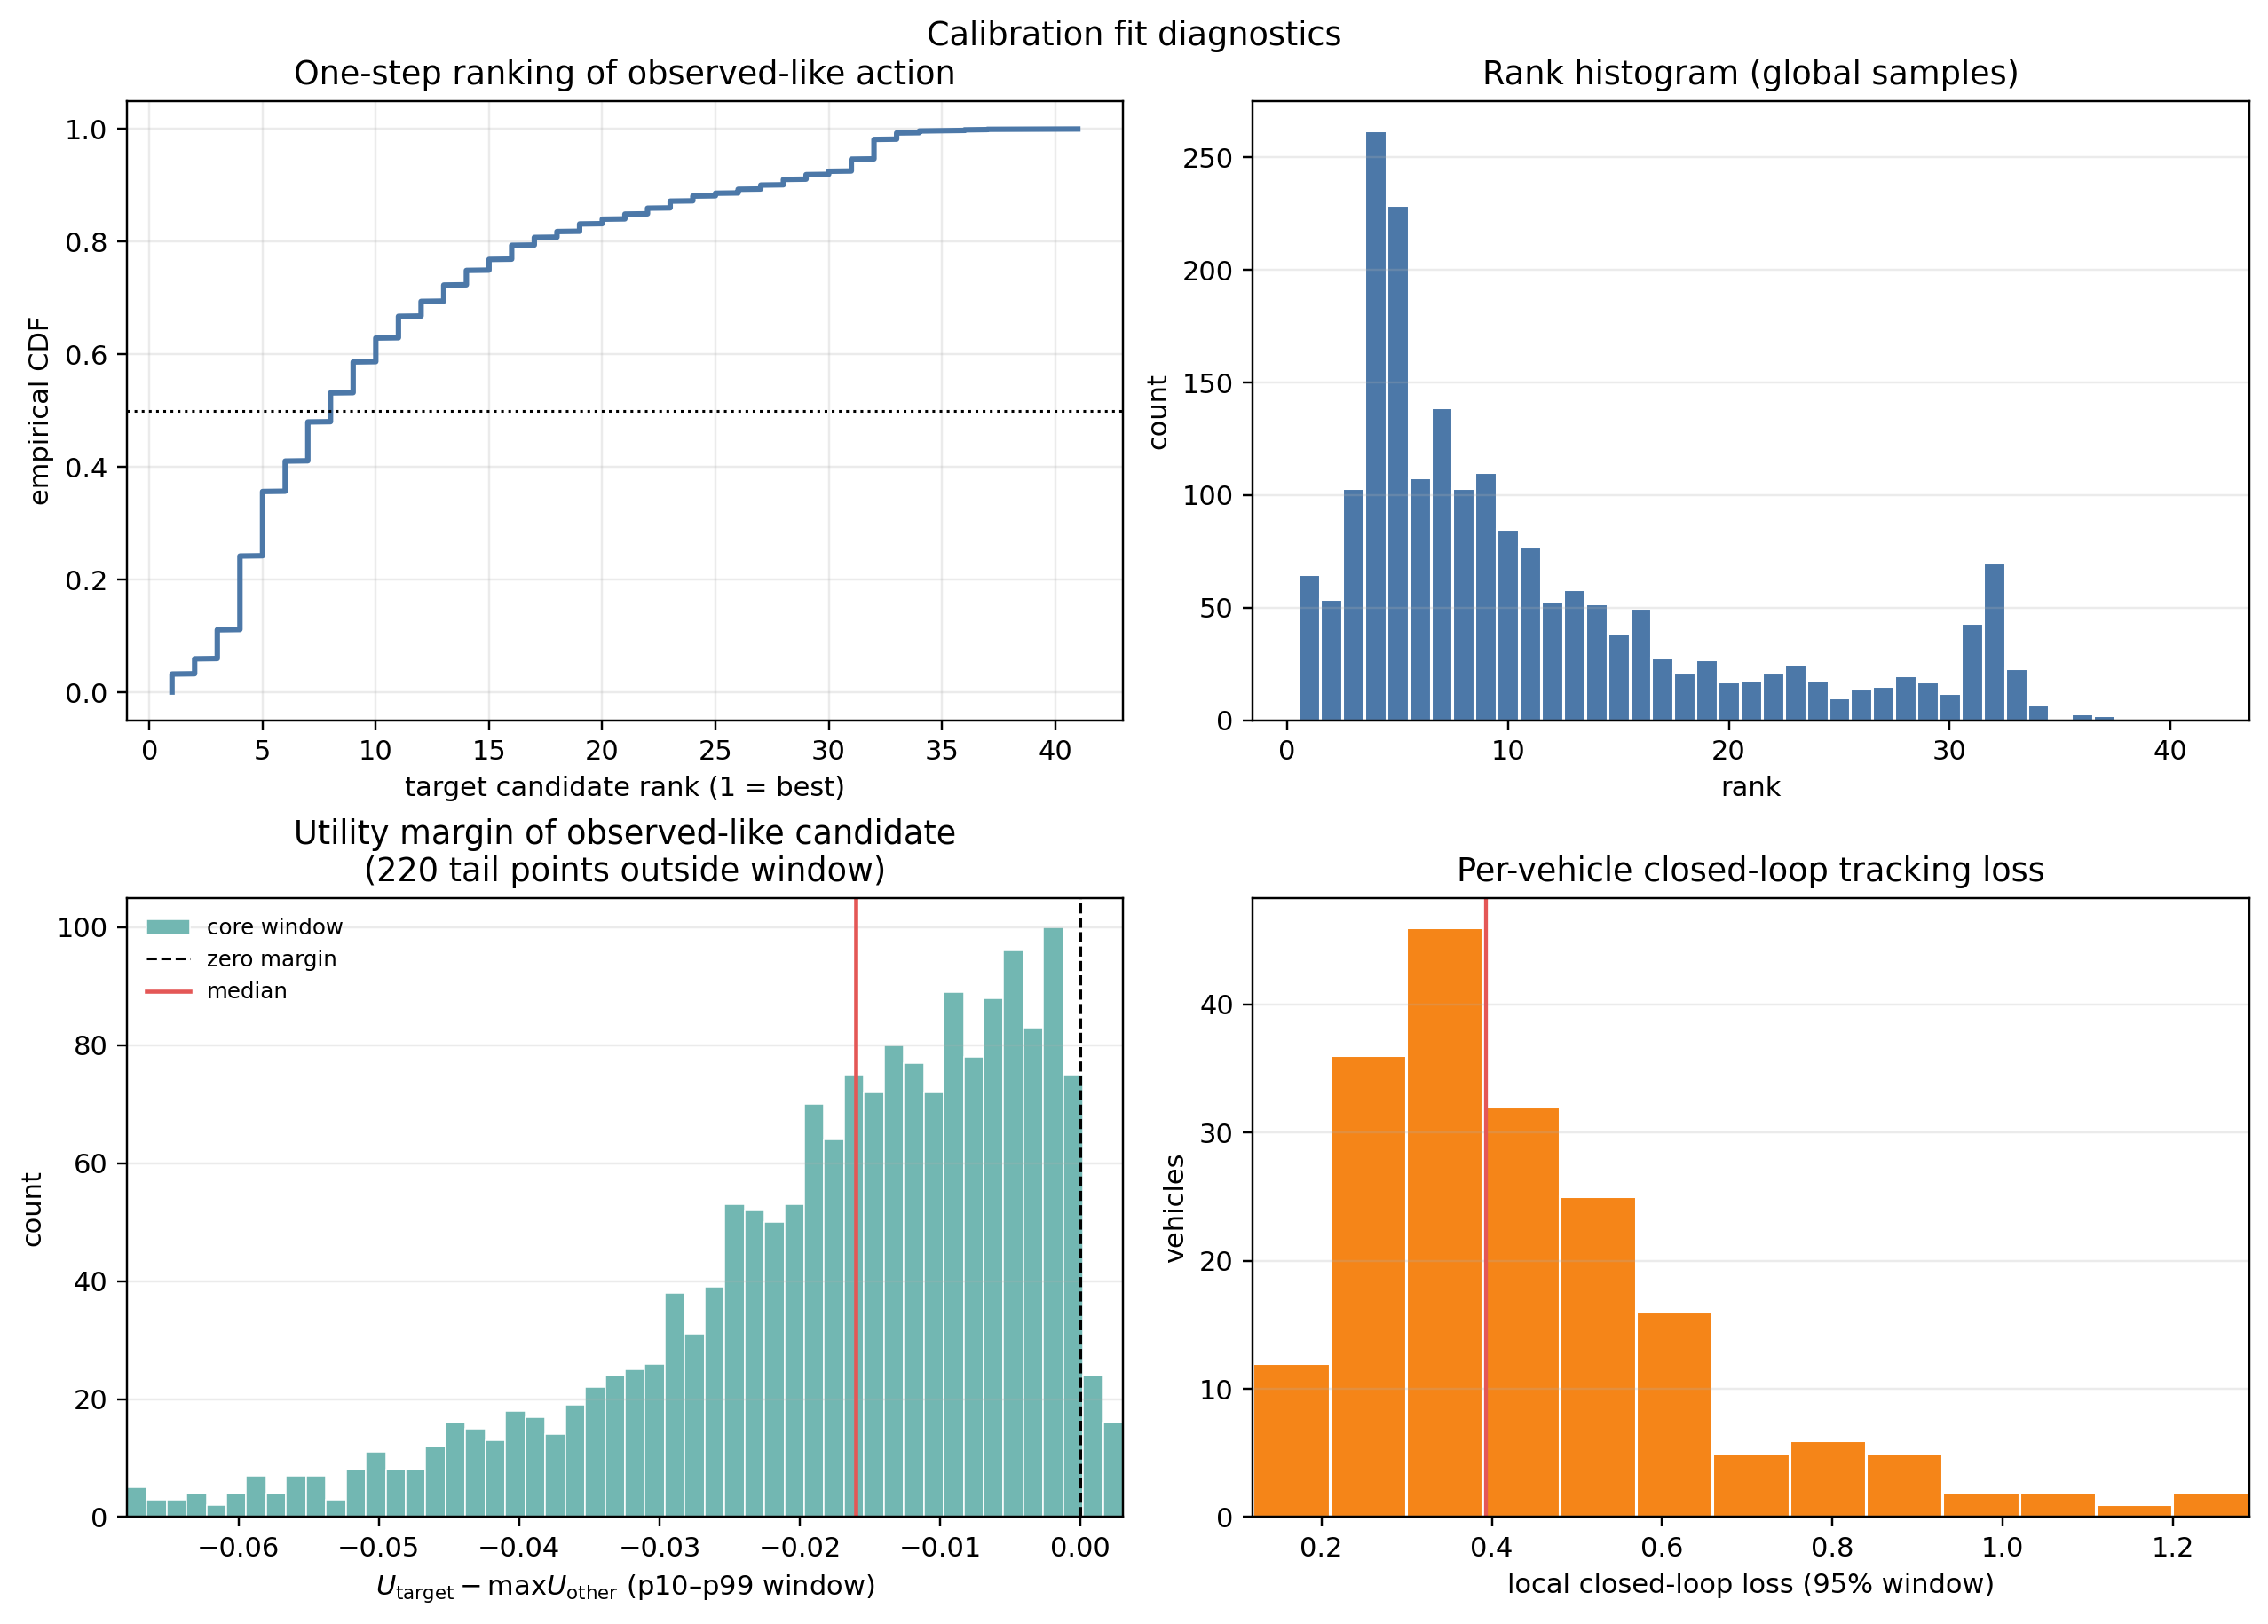
\includegraphics[width=\linewidth]{fig_fit_quality.png}
\caption{Calibration fit diagnostics: empirical CDF and histogram of the observed-like candidate rank, utility margin relative to the best alternative (core p10--p99 window), and per-vehicle closed-loop tracking loss.}
\label{fig:calibration_fit_quality}
\end{figure}

\paragraph{Working parameters and uncertainty.}
Table~\ref{tab:utility_calibration_params} reports the single best vector, the robust working point, top-cloud percentiles, and per-vehicle $95\%$ intervals. We recommend $\theta_{\mathrm{rob}}$ for all downstream simulation and residual learning:
\[
\begin{aligned}
&S_\theta=4.22,\ 
S_v=3.36,\ 
\xi_i=4.07,\ 
S_d=5.80,\ 
\gamma=1.45,\\
&w_x=5.45,\ 
w_y=3.91,\ 
w_c=374,\ 
w_\ell=44.2,\ 
\beta=1.93.
\end{aligned}
\]
Relative to $\theta^\star$, the robust set pulls extreme boundary values inward (notably $w_y$, $w_c$, and $\beta$), which is consistent with a flatter objective ridge rather than a unique sharp minimum. Fig.~\ref{fig:calibration_param_dist} shows the global scored-trial distributions (histogram and KDE restricted to the central $95\%$ mass), and Fig.~\ref{fig:calibration_param_dist_per_id} reports the corresponding per-vehicle local-fit distributions.

\begin{figure}[t]
\centering
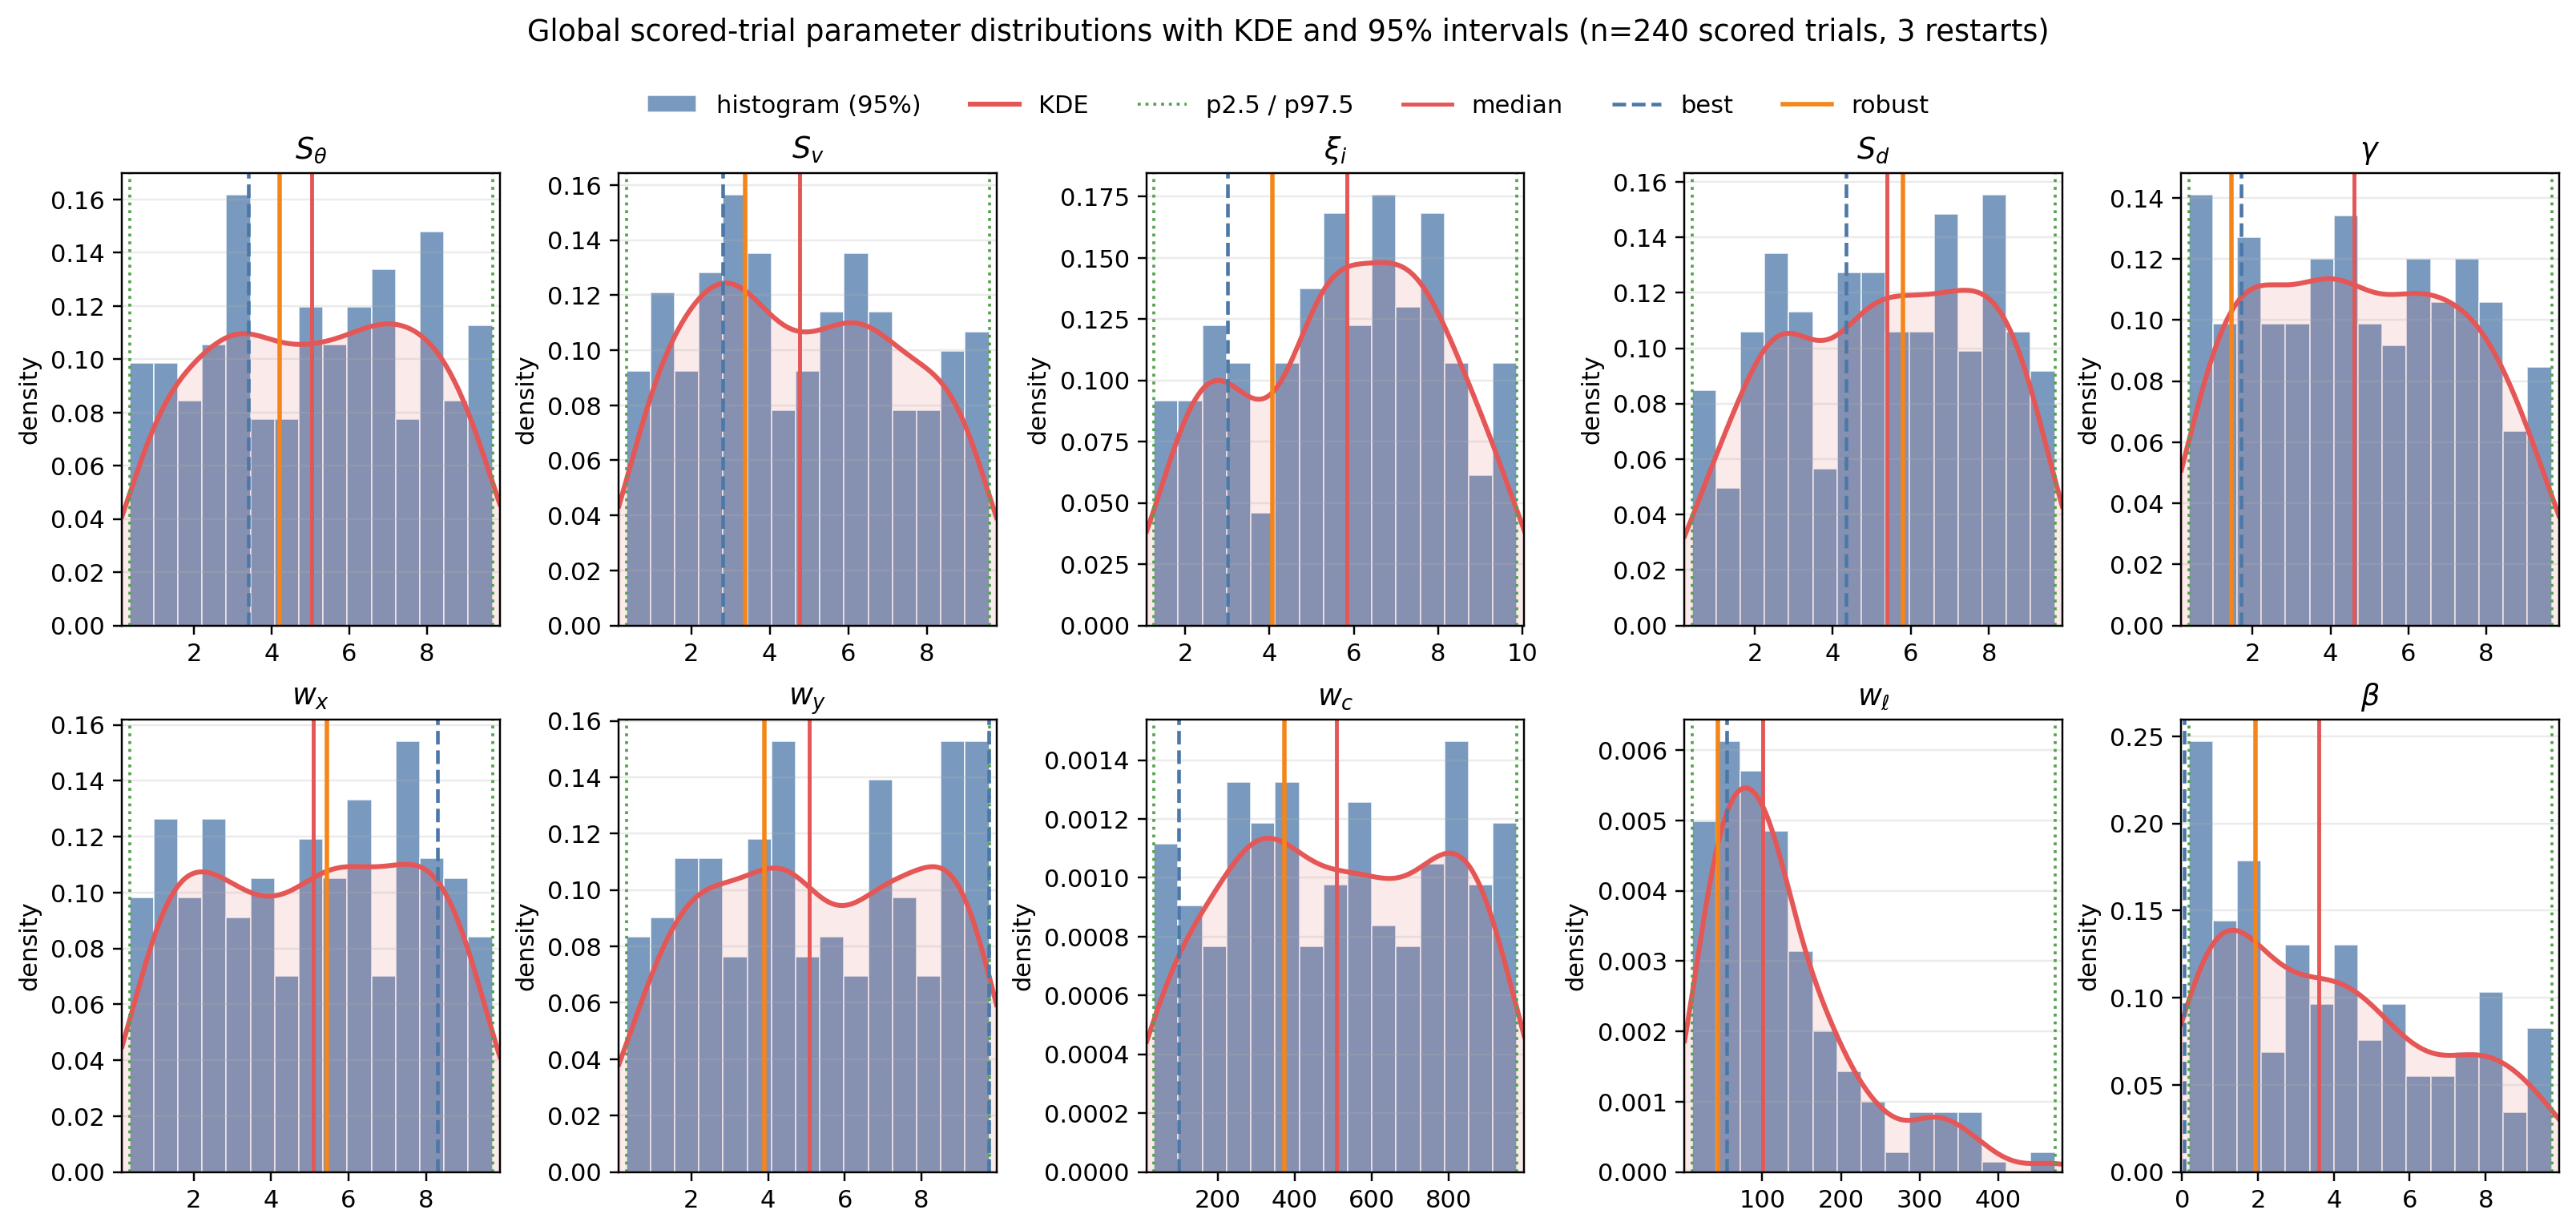
\includegraphics[width=\linewidth]{fig_parameter_distributions.png}
\caption{Global scored-trial distributions of the ten utility parameters ($240$ closed-loop-scored trials from three restarts). Histograms and KDEs are computed inside each parameter's central $95\%$ interval; vertical markers indicate the median, best, and robust values when they fall in that window.}
\label{fig:calibration_param_dist}
\end{figure}

\begin{figure}[t]
\centering
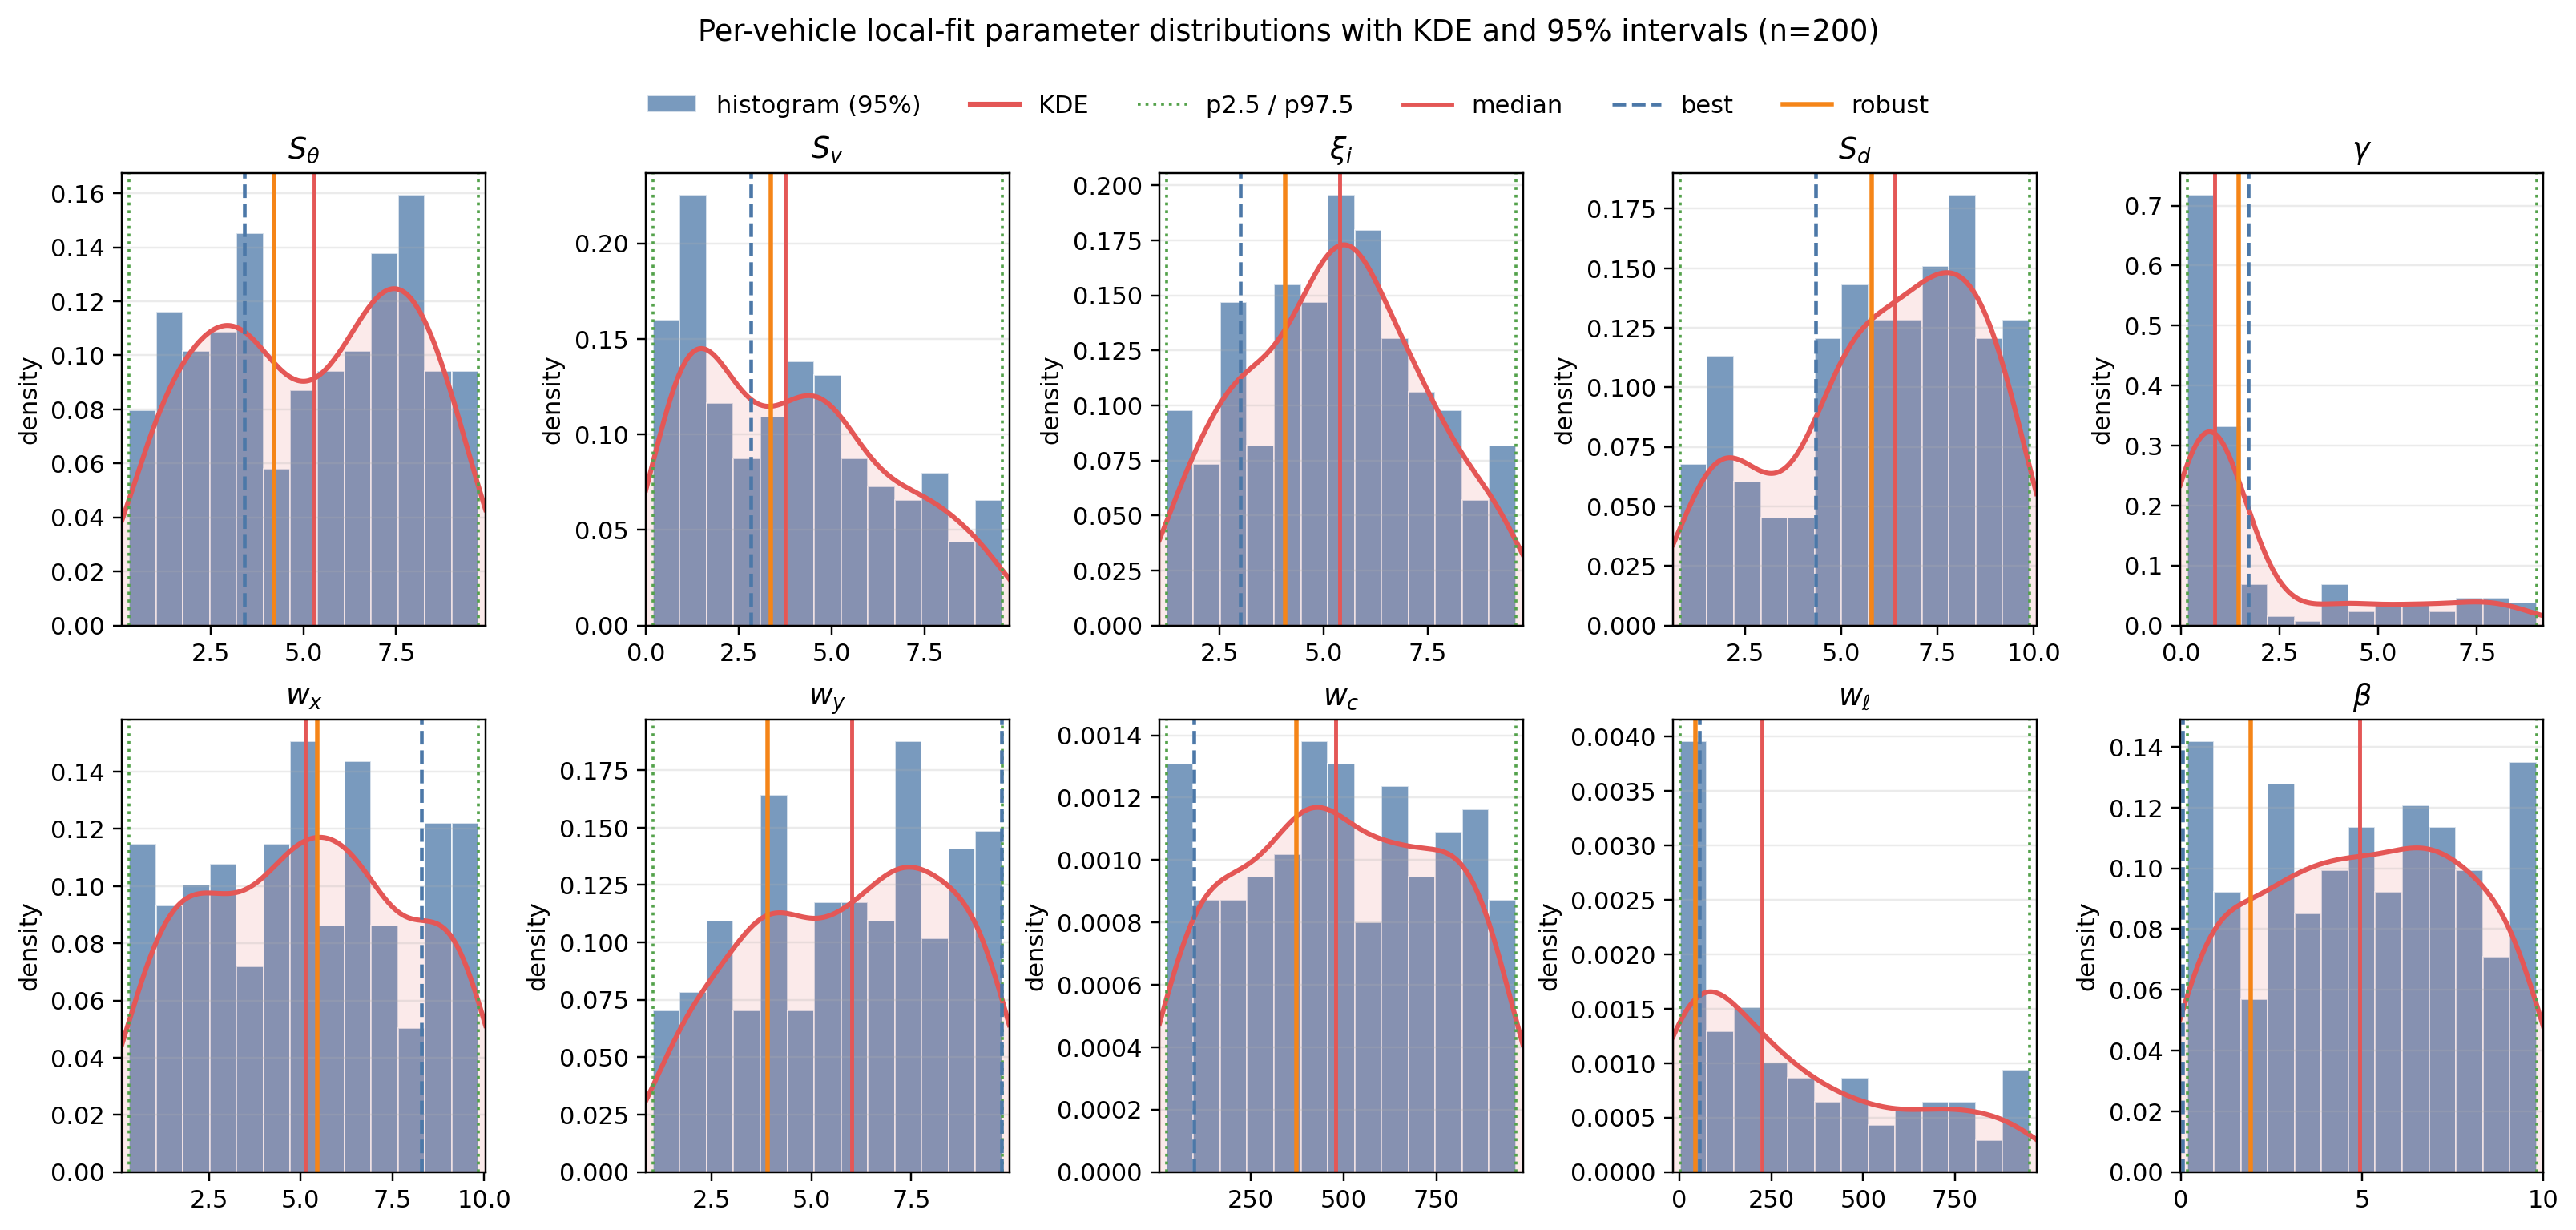
\includegraphics[width=\linewidth]{fig_parameter_distributions_per_id.png}
\caption{Per-vehicle local-fit parameter distributions ($200$ trajectories). Histograms and KDEs use the central $95\%$ mass for each coordinate.}
\label{fig:calibration_param_dist_per_id}
\end{figure}

\begin{figure}[t]
\centering
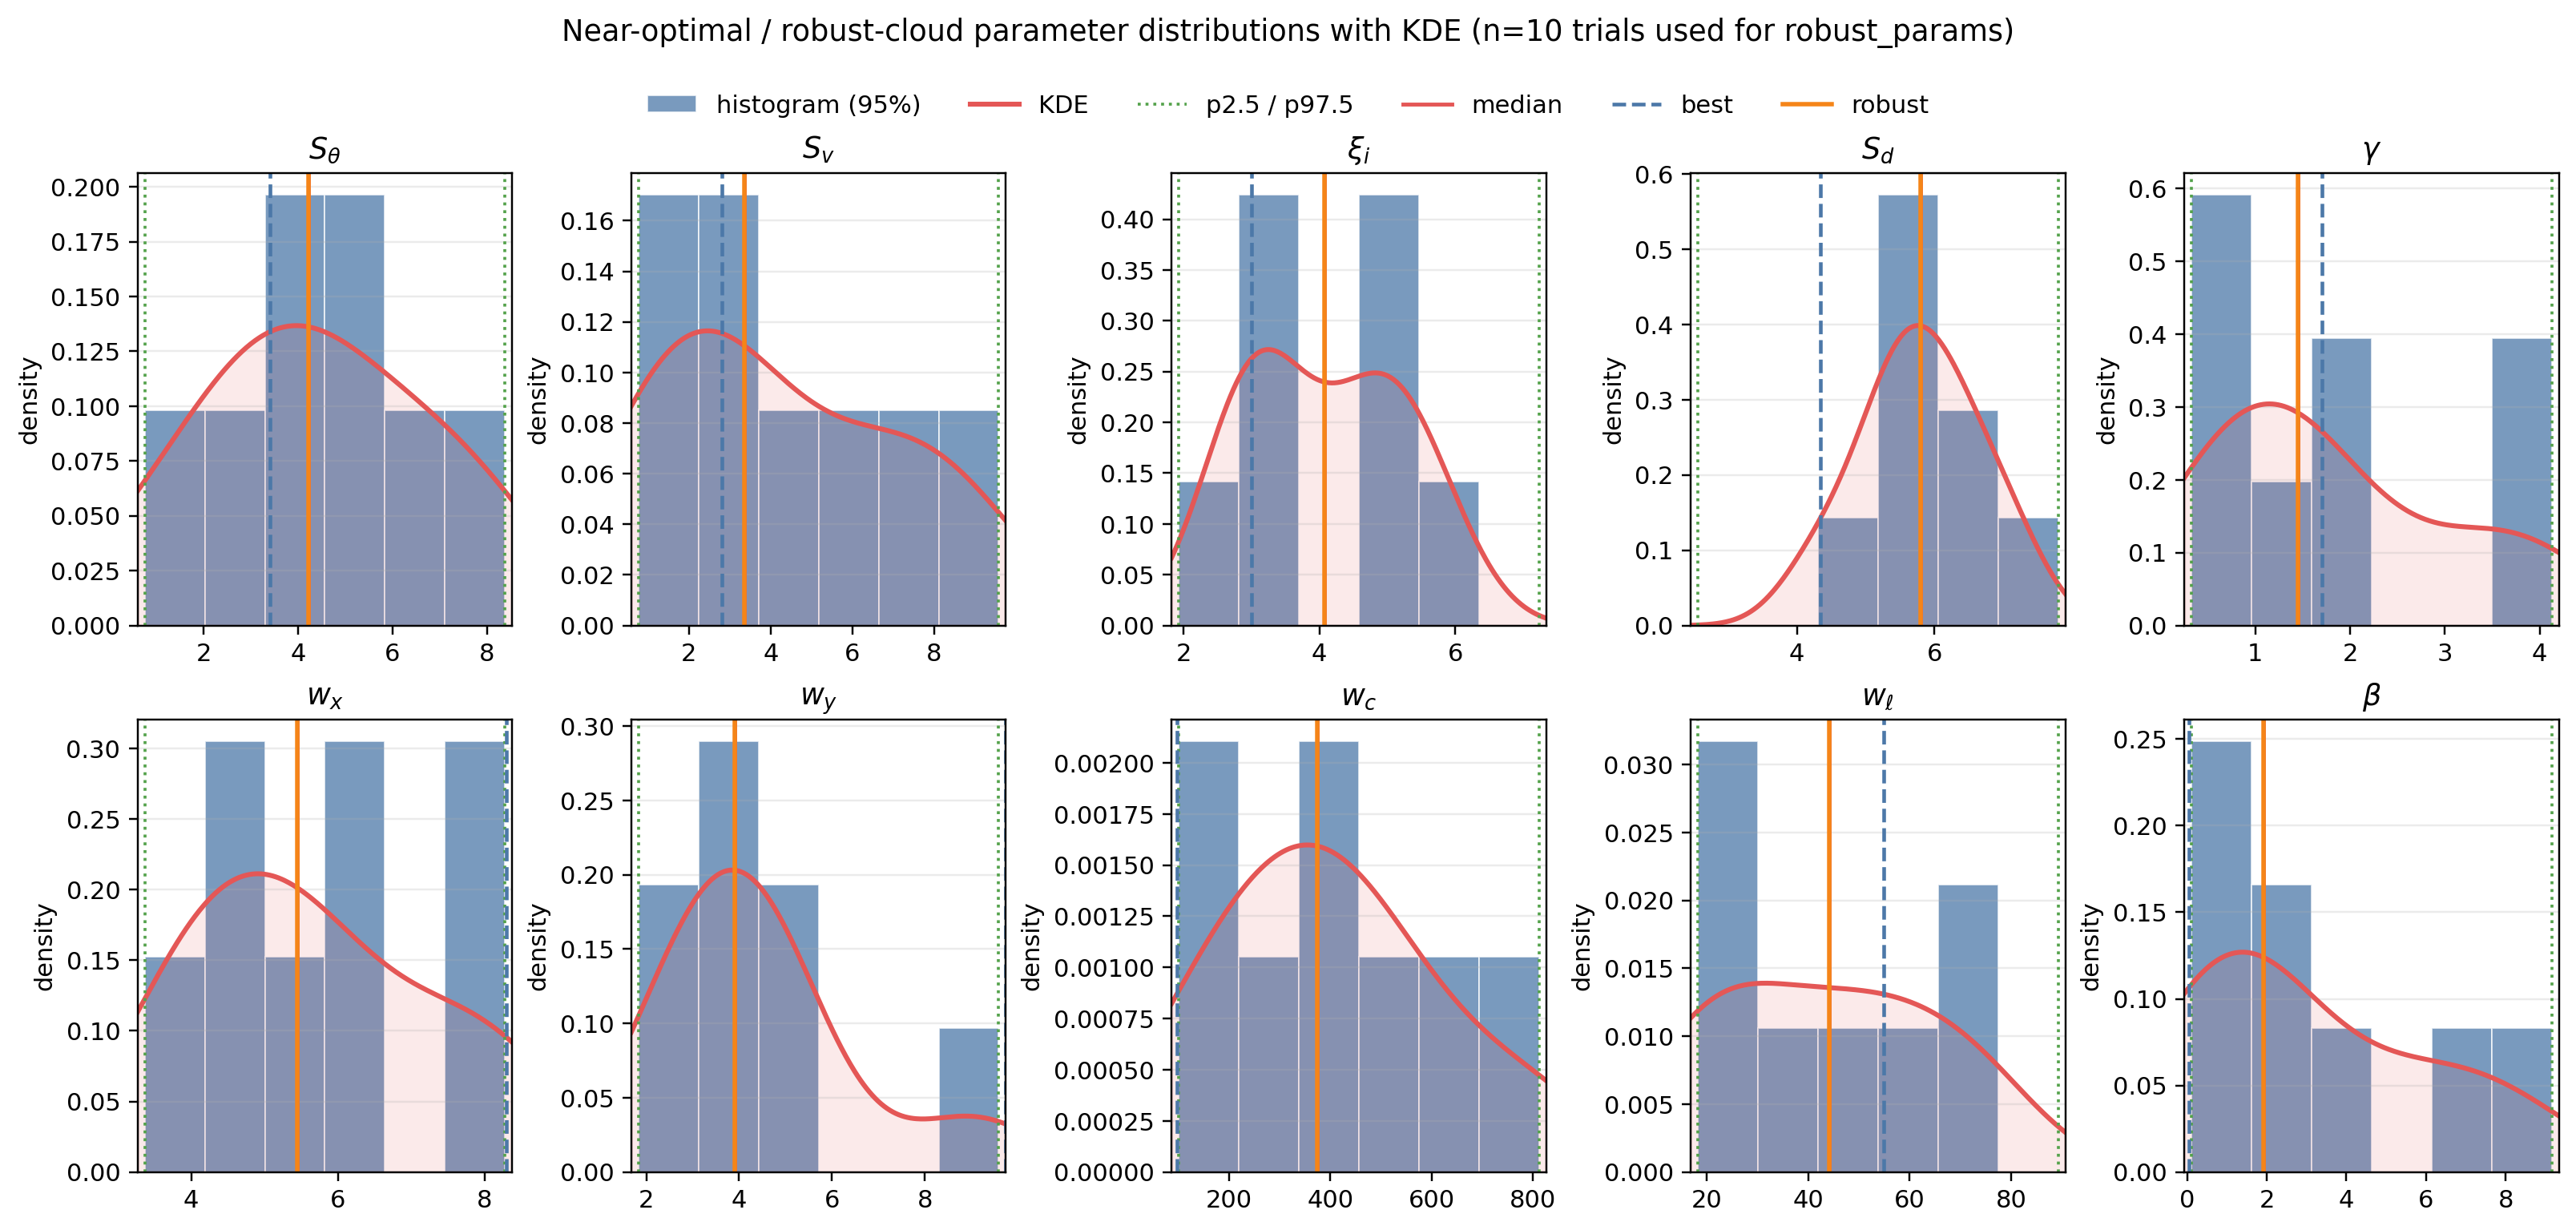
\includegraphics[width=\linewidth]{fig_parameter_distributions_near_optimal.png}
\caption{Parameter distributions over the near-optimal / top cloud used to form the robust working point $\theta_{\mathrm{rob}}$ (coordinate-wise median).}
\label{fig:calibration_param_dist_robust}
\end{figure}

\paragraph{Identifiability.}
Of $240$ closed-loop-scored trials, only a small subset lies near $J(\theta^\star)$; the near-optimal/top cloud still exhibits large coefficient-of-variation across most coordinates (Fig.~\ref{fig:calibration_identifiability}). The strongest tradeoff is between $S_v$ and $\gamma$ (correlation $-0.85$), with additional coupling among $(S_\theta,S_v)$, $(w_x,w_c)$, and $(w_c,w_\ell)$. Thus the data identify a \emph{region} of acceptable utility weights more reliably than a unique point estimate.

\begin{figure}[t]
\centering
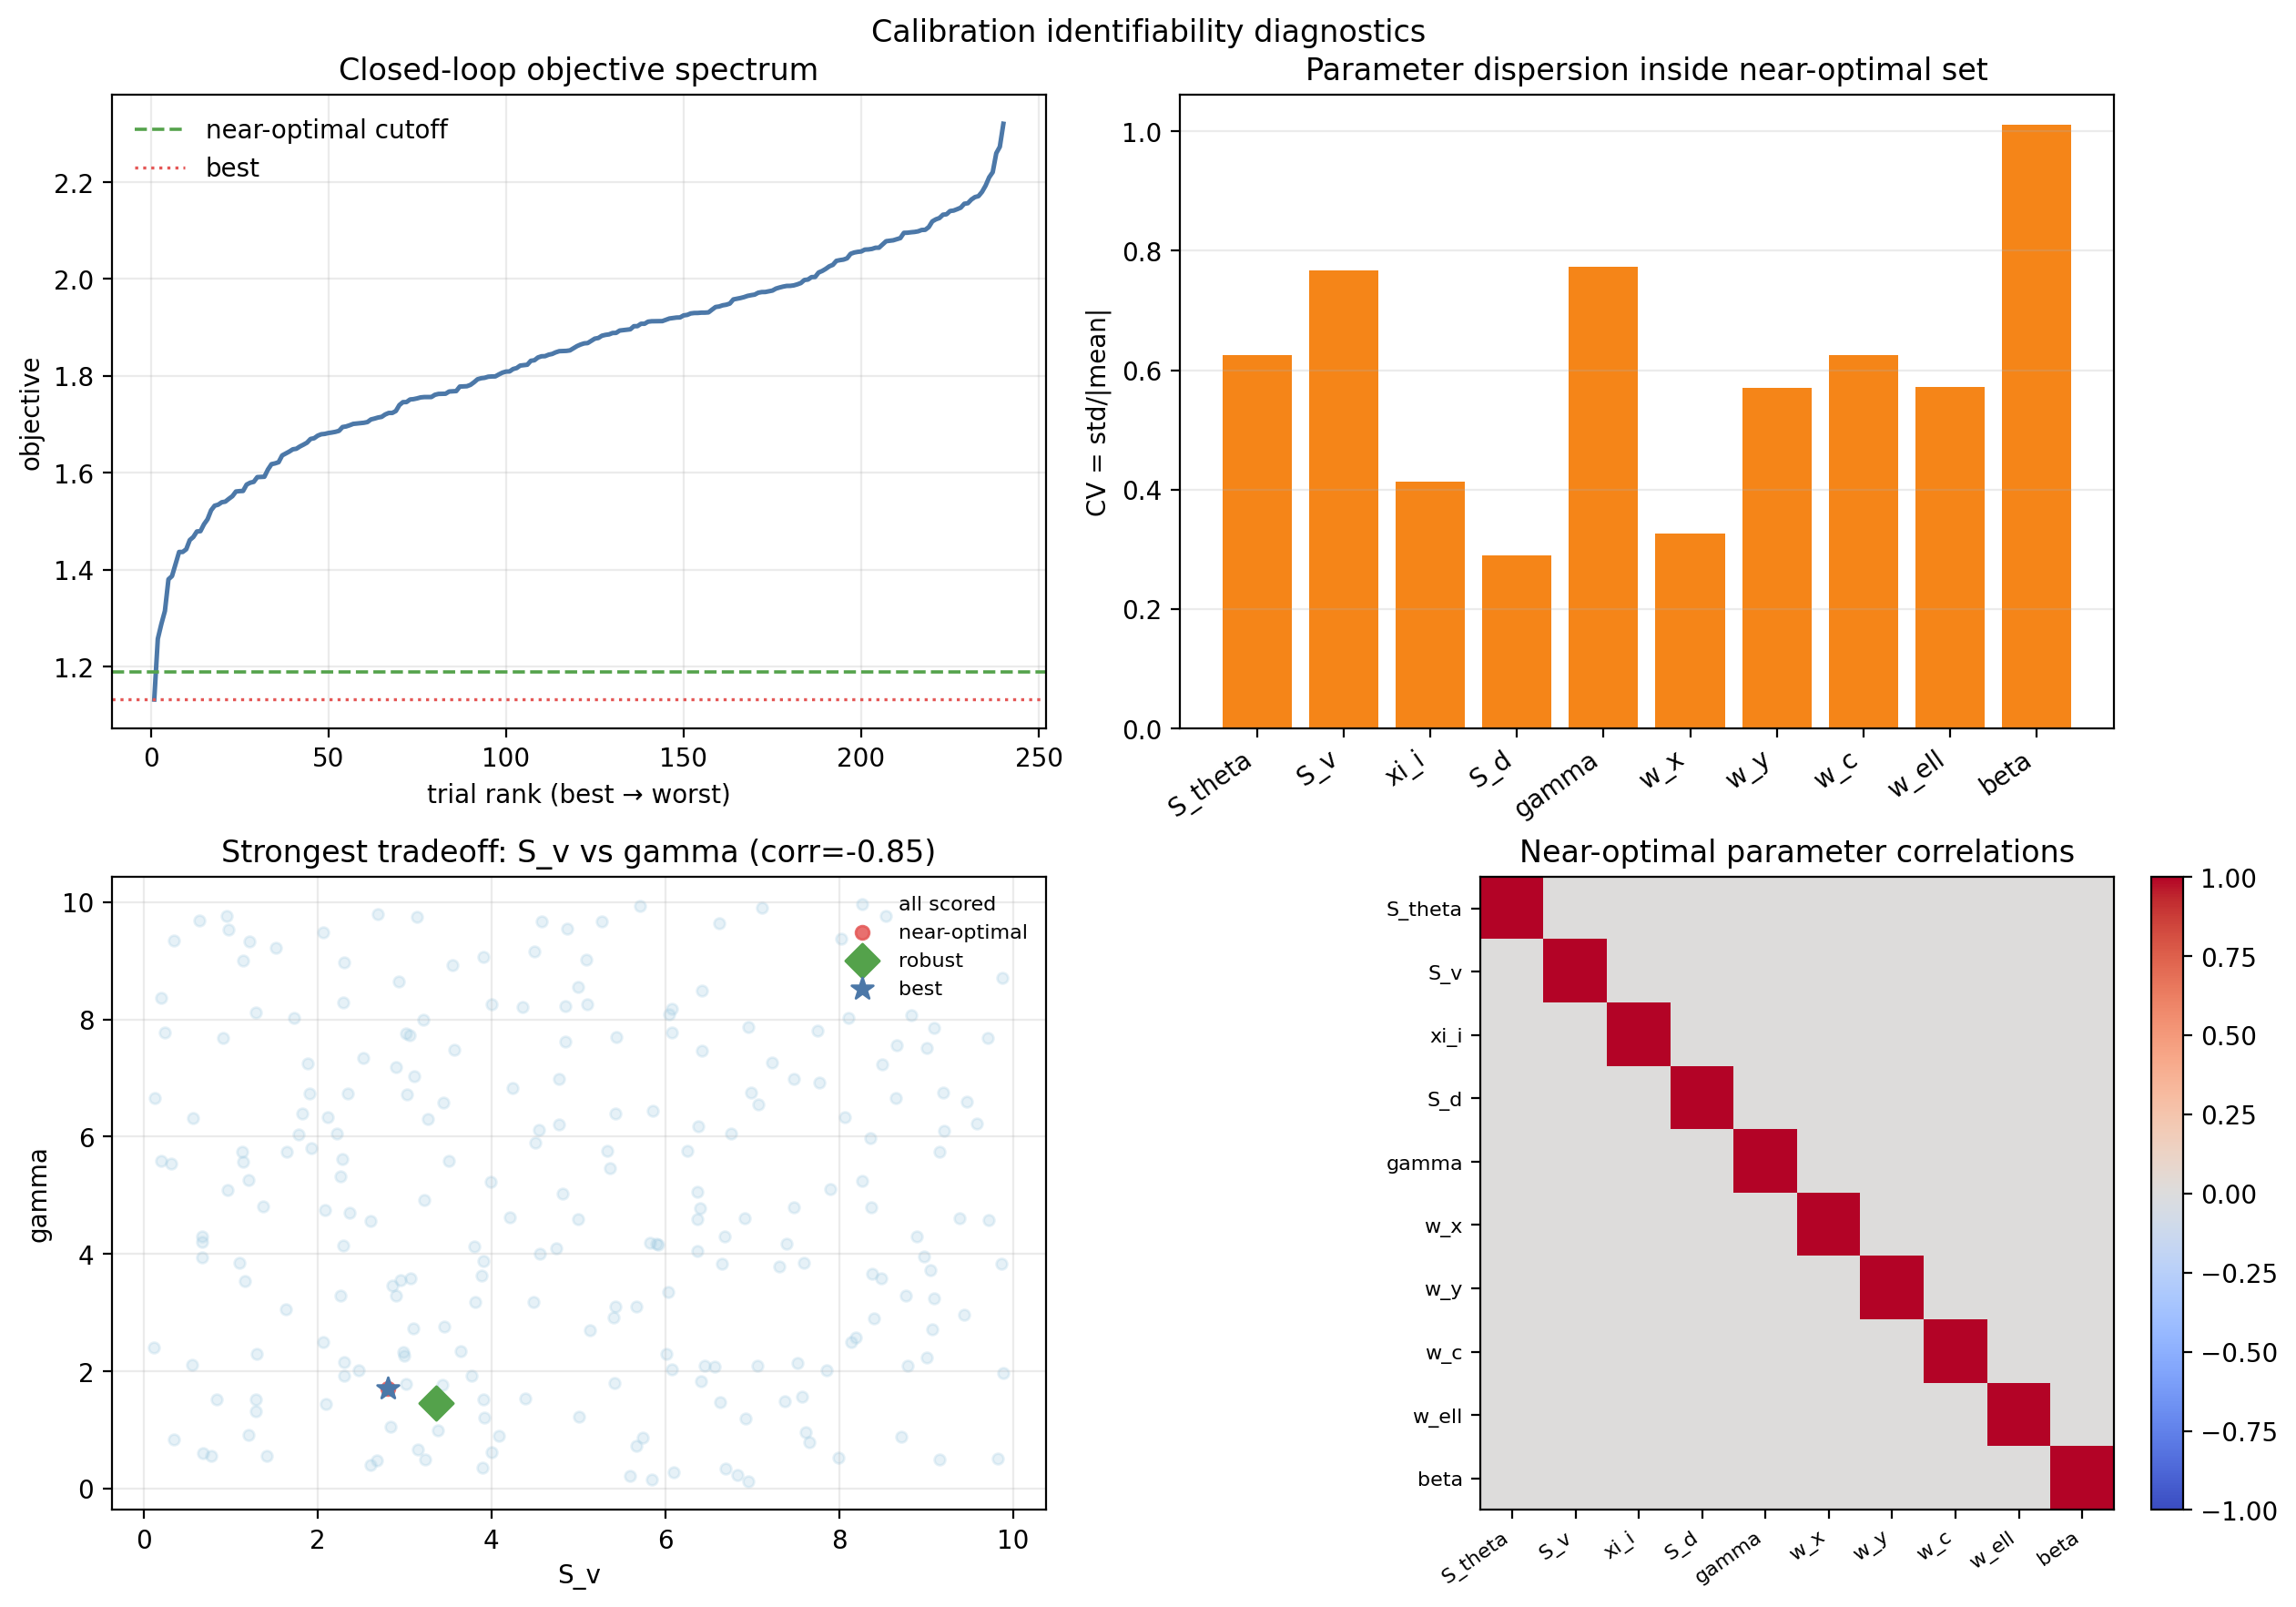
\includegraphics[width=\linewidth]{fig_identifiability_diagnostics.png}
\caption{Identifiability diagnostics: objective spectrum over ranked trials, coefficient of variation inside the near-optimal/top cloud, strongest pairwise tradeoff ($S_v$ versus $\gamma$), and near-optimal parameter correlation heatmap.}
\label{fig:calibration_identifiability}
\end{figure}

\paragraph{Implications.}
For the remainder of this paper we (i)~fix $\theta_{\mathrm{rob}}$ as the nominal utility prior, (ii)~use the reported percentile ranges as bounds for global sensitivity analysis, and (iii)~interpret residual policy learning as refining behavior within an already plausible, but non-unique, utility basin.

\begin{table}[t]
\centering
\caption{Calibrated utility parameters: best trial, robust median of the near-optimal/top cloud, top-cloud $p_{50}$/$p_{95}$, and per-vehicle local-fit median with central $95\%$ interval.}
\label{tab:utility_calibration_params}
\begin{tabular}{lrrrrrr}
\toprule
Param. & Best & Robust & Top $p_{50}$ & Top $p_{95}$ & Per-ID $p_{50}$ & Per-ID $95\%$ CI \\
\midrule
$S_\theta$ & $3.411$ & $4.216$ & $4.216$ & $8.299$ & $5.297$ & $[0.295,\,9.728]$ \\
$S_v$      & $2.809$ & $3.364$ & $3.364$ & $9.325$ & $3.737$ & $[0.182,\,9.585]$ \\
$\xi_i$    & $3.000$ & $4.074$ & $4.074$ & $6.791$ & $5.373$ & $[1.227,\,9.609]$ \\
$S_d$      & $4.343$ & $5.802$ & $5.802$ & $7.604$ & $6.393$ & $[0.818,\,9.890]$ \\
$\gamma$   & $1.700$ & $1.453$ & $1.453$ & $4.048$ & $0.854$ & $[0.155,\,9.009]$ \\
$w_x$      & $8.297$ & $5.449$ & $5.449$ & $8.257$ & $5.121$ & $[0.322,\,9.850]$ \\
$w_y$      & $9.747$ & $3.906$ & $3.906$ & $9.439$ & $6.015$ & $[1.030,\,9.774]$ \\
$w_c$      & $97.45$ & $373.9$ & $373.9$ & $807.7$ & $477.8$ & $[23.2,\,963.7]$ \\
$w_\ell$   & $54.91$ & $44.16$ & $44.16$ & $84.73$ & $225.3$ & $[2.41,\,952.5]$ \\
$\beta$   & $0.047$ & $1.925$ & $1.925$ & $8.878$ & $4.941$ & $[0.172,\,9.810]$ \\
\bottomrule
\end{tabular}
\end{table}

% --- Paste into Limitations (or keep as a short subsection) ---
Although the calibrated utility prior provides a usable working point for residual learning, several limitations should be noted. First, the ten-dimensional utility parameter vector is only weakly identified: multiple substantially different parameter combinations attain nearly the same closed-loop objective, with strong tradeoffs such as that between \(S_v\) and \(\gamma\). Consequently, the calibration identifies a region of acceptable behavior rather than a unique optimum, which is why we report a robust median of near-optimal trials together with percentile ranges instead of relying on a single best vector. Second, one-step ranking remains imperfect on the discrete candidate grid---the observed-like action is frequently competitive (median rank near eight; top-ten hit rate about \(63\%\)) but is rarely selected as the unique maximizer---so the one-step likelihood alone under-constrains the parameters and must be complemented by short-horizon closed-loop tracking. Third, per-vehicle local fits exhibit wide dispersion, indicating residual heterogeneity that a single population prior cannot fully capture. Finally, global sensitivity conclusions are meaningful only when Sobol ranges are aligned with the calibrated uncertainty region; using substantially narrower ad-hoc bounds can understate (or misattribute) parameter influence relative to the operating regime used downstream.
